\begin{figure}[htb]
\captionsetup[subfigure]{font={bf,large}, skip=1pt, margin=-0.7cm,justification=raggedright, singlelinecheck=false}
 \centering
\begin{subcaptionblock}{0.3\linewidth}
 \subcaption{}\label{fig:mechanism:1}
  \includegraphics[width=\textwidth]{fig_1_1_mechanism/schematic_orientation.v.0.2.0.pdf} 
\end{subcaptionblock}
\begin{subcaptionblock}{0.3\linewidth}
 \subcaption{}\label{fig:mechanism:2}
  \includegraphics[width=\textwidth]{fig_1_1_mechanism/schematic_atomic.v.0.2.0.pdf} 
\end{subcaptionblock}
\begin{subcaptionblock}{0.3\linewidth}
 \subcaption{}\label{fig:mechanism:3}
  \includegraphics[width=\textwidth]{fig_1_1_mechanism/schematic_electronic.v.0.2.0.pdf} 
\end{subcaptionblock}
%  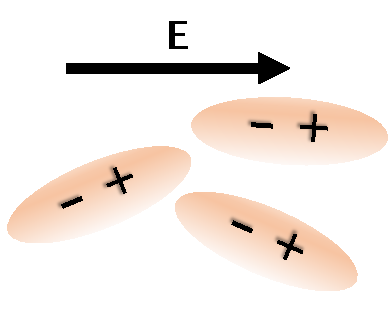
\includegraphics[]{figures/fig_mechanism/orientational_polarization.pdf}  
%  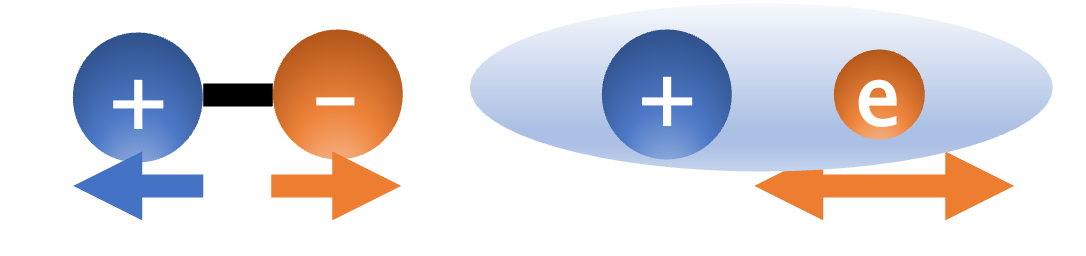
\includegraphics[]{figures/fig_mechanism/mechanism.png}
  \caption{The schematic image of three physical mechanisms of (a) the orientational (b) atomic (c) electronic polarization. $\vb{E}$ denotes the external electric field, and these diagrams show how the system changes before and after the electric field is applied.}
\label{Fig:mechanism}
\end{figure}
